\documentclass[11pt]{article}
\usepackage{amssymb, amsthm, amsmath}
\usepackage{bm}
\usepackage{graphicx}
\usepackage[authoryear]{natbib}
\usepackage{bm}
\usepackage{verbatim}
\usepackage{lineno}
\usepackage{times}
\usepackage{soul}
\usepackage{color}

\usepackage[left=1in,top=1in,right=1in]{geometry}
\pdfpageheight 11in
\pdfpagewidth 8.5in
\linespread{1.0}
\newcommand{\btheta}{ \mbox{\boldmath $\theta$}}
\newcommand{\bmu}{ \mbox{\boldmath $\mu$}}
\newcommand{\balpha}{ \mbox{\boldmath $\alpha$}}
\newcommand{\bbeta}{ \mbox{\boldmath $\beta$}}
\newcommand{\bdelta}{ \mbox{\boldmath $\delta$}}
\newcommand{\blambda}{ \mbox{\boldmath $\lambda$}}
\newcommand{\bgamma}{ \mbox{\boldmath $\gamma$}}
\newcommand{\brho}{ \mbox{\boldmath $\rho$}}
\newcommand{\bpsi}{ \mbox{\boldmath $\psi$}}
\newcommand{\bepsilon}{ \mbox{\boldmath $\epsilon$}}
\newcommand{\bomega}{ \mbox{\boldmath $\omega$}}
\newcommand{\bOmega}{ \mbox{\boldmath $\Omega$}}
\newcommand{\bDelta}{ \mbox{\boldmath $\Delta$}}
\newcommand{\bSigma}{ \mbox{\boldmath $\Sigma$}}
\newcommand{\bPsi}{\mbox{\boldmath $\Psi$}}
\newcommand{\bOne}{\mbox{\boldmath $1$}}
\newcommand{\omu}{\overline{\mu}}
\newcommand{\oSigma}{\overline{\Sigma}}
\newcommand{\Yt}{{\tilde Y}}
\newcommand{\bA}{ \mbox{\bf A}}
\newcommand{\bP}{ \mbox{\bf P}}
\newcommand{\bx}{ \mbox{\bf x}}
\newcommand{\bX}{ \mbox{\bf X}}
\newcommand{\bB}{ \mbox{\bf B}}
\newcommand{\bZ}{ \mbox{\bf Z}}
\newcommand{\by}{ \mbox{\bf y}}
\newcommand{\bY}{ \mbox{\bf Y}}
\newcommand{\bz}{ \mbox{\bf z}}
\newcommand{\bh}{ \mbox{\bf h}}
\newcommand{\br}{ \mbox{\bf r}}
\newcommand{\bt}{ \mbox{\bf t}}
\newcommand{\bs}{ \mbox{\bf s}}
\newcommand{\bb}{ \mbox{\bf b}}
\newcommand{\bL}{ \mbox{\bf L}}
\newcommand{\bu}{ \mbox{\bf u}}
\newcommand{\bv}{ \mbox{\bf v}}
\newcommand{\bV}{ \mbox{\bf V}}
\newcommand{\bW}{ \mbox{\bf W}}
\newcommand{\bG}{ \mbox{\bf G}}
\newcommand{\bH}{ \mbox{\bf H}}
\newcommand{\bw}{ \mbox{\bf w}}
\newcommand{\bo}{ \mbox{\bf o}}
\newcommand{\bfe}{ \mbox{\bf e}}
\newcommand{\iid}{\stackrel{iid}{\sim}}
\newcommand{\indep}{\stackrel{indep}{\sim}}
\newcommand{\calR}{{\cal R}}
\newcommand{\calG}{{\cal G}}
\newcommand{\calD}{{\cal D}}
\newcommand{\calS}{{\cal S}}
\newcommand{\calB}{{\cal B}}
\newcommand{\calA}{{\cal A}}
\newcommand{\calT}{{\cal T}}
\newcommand{\calO}{{\cal O}}
\newcommand{\argmax}{{\mathop{\rm arg\, max}}}
\newcommand{\argmin}{{\mathop{\rm arg\, min}}}
\newcommand{\Frechet}{\mbox{Fr$\acute{\mbox{e}}$chet }}
\newcommand{\Matern}{\mbox{Mat$\acute{\mbox{e}}$rn }}
\newcommand{\ballunion}{B_a(\bs_1) \cup B_b(\bs_2) }

\newcommand{\beq}{ \begin{equation}}
\newcommand{\eeq}{ \end{equation}}
\newcommand{\beqn}{ \begin{eqnarray}}
\newcommand{\eeqn}{ \end{eqnarray}}


\begin{document}\linenumbers

\begin{center}
{\Large {\bf A new spatial model for points above a threshold}}\\
\today
\end{center}

\section{Introduction}\label{s:intro}
In most climatological applications, researchers are interested in learning about the average behavior of different climate variables (e.g. ozone, temperature, rainfall).
However, averages do not help regulators prepare for the unusual events that only happen once every 100 years.
For example, it is important to have an idea of how much rain will come in a 100-year floor in order to construct strong enough river levees to protect lands from flooding.

Unlike multivariate normal distributions, it is challenging to model multivariate extreme value distributions (e.g. generalized extreme value and generalized Pareto distribution) because few closed-form expressions exist for the density in more than two-dimensions \citep{Coles1991}.
Given this limitation, pairwise composite likelihoods have been used when modeling dependent extremes \citep{Padoan2010,Blanchet2011,Huser2013}.

One way around the multi-dimensional limitation of multivariate extreme value distributions is to use skew elliptical distributions to model dependent extreme values \citep{Genton2004,Zhang2010,Padoan2011}.
Due to their flexibility, the skew-normal and skew-$t$ distribution offer a flexible way to handle non-symmetric data within a framework of multivariate normal and multivariate t-distributions.
As with the spatial Gaussian process, the skew-normal distribution is also asymptotically independent; however, the skew-$t$ does demonstrate asymptotic dependence \citep{Padoan2011}.
Although asymptotic dependence is desirable between sites that are near one another, one drawback to the skew-$t$ is that sites remain asymptotically dependent even at far distances.

In this paper, we present a model that has marginal distributions with flexible tails, demonstrates asymptotic dependence for observations at sites that are near to one another, and has computation on the order of Gaussian models for large space-time datasets.
Specifically, our contribution is to incorporate thresholding and random spatial partitions using a multivariate skew-$t$ distribution.
The advantage of using a thresholded model as opposed to a non-thresholded model is that is allows for the tails of the distribution to inform the predictions in the tails \citep{DuMouchel1983}.
The random spatial partition alleviates the long-range spatial dependence seen by the skew-$t$.

The paper is organized as follows.
Section \ref{s:skewt} is a brief review of the spatial skew-$t$ process.
In section \ref{s:temporal}, we build upon the traditional skew-$t$ by incorporating censoring to focus on tails, partitioning to remove long-range asymptotic dependence, and extending the model to space-time data.
The computing is described in section \ref{s:comp}.
In section \ref{s:simstudy}, we present a simulation study that examines the predictive capabilities of this model compared with a na{\"i}ve Gaussian method.
We then compare our method to Gaussian and max-stable methods with a data analysis of ozone measurements from the eastern US in section \ref{s:analysis}.
The final section provides brief discussion and direction for future research.

\section{Spatial skew processes}\label{s:spatialskew}
Many types of data demonstrate some level of skewness and therefore should be modeled with distributions that allow for asymmetry.
The skew-elliptical family of distributions provides models that are mathematically tractable while introducing a slant parameter to account for asymmetric data \citep{Genton2004}.
A brief review of the additive process by which a skew-$t$ process is created is given here.

\subsection{Skew-$t$ process} \label{s:skewt}
Let $Y(\bs)$ be the observation at spatial location $\bs = (s_1, s_2)$.
The spatial skew-$t$ process can be written
\begin{align}
  Y(\bs) = \bX(\bs)^T \bbeta + \lambda \sigma |z| + \sigma v(\bs)
\end{align}
where $\bX(\bs)$ is a set of spatial covariates at site $\bs$, $\bbeta$ is a set of regression parameters, $\lambda \in \calR$ is a parameter controlling skew, $z \sim N(0, 1)$, $\sigma^2 \sim \text{IG}(a, b)$ is an inverse gamma random variable, and $v(\bs)$ is a spatial Gaussian process with mean zero and variance one.
A common spatial correlation function is the \Matern with
\begin{align}
  \text{cor}(v(\bs), v(\bt)) = \gamma I(\bs = \bt) + (1 - \gamma)  \frac{ 1 }{ \Gamma(\nu) 2^{ \nu - 1}} \left( \sqrt{2\nu} \frac{ h }{ \rho } \right)^{\nu} K_{\nu} \left( \sqrt{2\nu} \frac{ h }{ \rho } \right) \label{eq:matern}
\end{align}
where $\rho$ is the spatial range, $\nu$ is the smoothness, $\gamma$ is the proportion of variance accounted for by the spatial variation, $K_\nu$ is a modified Bessel function of the second kind, and $h = || \bs - \bt ||$.

Let $\bY = [Y(\bs_1), \ldots, Y(\bs_n)]^T$ be a set of observations at a finite collection of locations $\bs_1, \ldots, \bs_n$.
After marginalizing over both $z$ and $\sigma$,
\begin{align}
  \bY \sim \text{ST}_n(\bX \bbeta, \bOmega, \balpha, 2a), \label{eq:fullmodel}
\end{align}
that is, $\bY$ follows an $n$-dimensional skew-$t$ process with location $\bX \bbeta$, correlation matrix $\bOmega$, slant parameters $\balpha$ and degrees of freedom $2a$, where $\bX = [\bX(\bs_1)^T, \ldots, \bX(\bs_n)^T]$, $\bOmega = \bomega \bar{\bOmega} \bomega$, $\bomega = \text{diag}\left(\frac{1}{ \sqrt{ab}}, \ldots, \frac{1}{\sqrt{ab}}\right)$, $\bar{\bOmega} = (\bSigma + \lambda^2 \bOne \bOne^T$), $\bSigma$ is a positive definite correlation matrix, $\balpha = \lambda (1 + \lambda^2 \bOne^T \bSigma^{-1} \bOne)^{-1/2} \bOne^T \bSigma^{-1}$ is a vector of slant parameters.
This process is desirable because of its flexible tail that is controlled by the skewness parameter $\lambda$ and degrees of freedom $2a$.
Furthermore, the marginal distributions at each location also follow a univariate skew-$t$ distribution \citep{Azzalini2013}.

\subsection{Extremal dependence}
One measure of extremal dependence is the $\chi$ statistic \citep{Padoan2011}.
The $\chi$ statistic for the upper tail is given by $\lim_{c \rightarrow \infty} \Pr(Y(\bs_1) > c | Y(\bs_2) > c)$.
For a stationary spatial process, we can write the $\chi$ coefficient as
\begin{align}
  \chi(h) = \lim_{c \rightarrow \infty} \Pr[Y(\bs) > c | Y(\bt) > c].
\end{align}
If $\chi(h) = 0$, then observations are asymptotically independent at distance $h$.
For Gaussian processes, $\chi(h) = 0$ regardless of the distance, so they are not suitable for modeling spatially-dependent extremes.
Unlike the Gaussian process, the skew-$t$ process is asymptotically dependent.
However, one problem with the spatial skew-$t$ process is that $\lim_{h \rightarrow \infty} \chi(h) > 0$.
This occurs because all observations, both near and far, share the same $z$ and $\sigma$ terms.
Therefore, the skew-$t$ process is not ideal for spatial analysis of large geographic regions where we expect only local spatial dependence.
The explicit expression for $\chi(h)$ \citep{Padoan2011} and a proof of this are given in Appendix \ref{a:skewt}.

\section{Spatiotemporal skew-$t$ model for extremes}\label{s:spatial}
In this section, we propose extensions to the skew-$t$ process to model spatial extremes over a large geographic region by introducing censoring to focus on tail behavior and a random partition similar to \citet{Kim2005} to remove long-range asymptotic dependence.

\subsection{Censoring to focus on the tails}
To avoid bias in estimating tail parameters, we model censored data.
Let
\beq\label{Yt}
  \tilde{Y}(\bs) = \left\{ \begin{array}{ll}
      Y(\bs) \quad & \delta(\bs) = 1 \\
      T & \delta(\bs) = 0
  \end{array} \right.
\eeq
be the censored observation at site $\bs$ where $Y(\bs)$ is the uncensored observation, $\delta(\bs) = I[Y(\bs) > T]$, and $T$ is a pre-specified threshold value.
Then, assuming the uncensored data $Y(\bs)$ are observations from a skew-$t$ process, we update values censored below the threshold using standard Bayesian missing data methods as described in Section \ref{s:comp}.

\subsection{Partitioning to remove long-range asymptotic dependence}\label{s:part}
We handle the problem of long-range asymptotic dependence with a random partition model.
As discussed in Section \ref{s:spatialskew}, the source of long-range dependence is the shared $z$ and $\sigma$.
Therefore, to alleviate this dependence, we allow $z$ and $\sigma$ to vary by site.
Then, the model becomes
\begin{align} \label{eq:partition}
  Y(\bs) &= \bX(\bs)^T \bbeta + \lambda \sigma(\bs) |z(\bs)| + \sigma(\bs) v(\bs).
\end{align}
Let $\bw = (w_1, w_2)$ be the location of a spatial knot.
To model spatial variation, consider a set of spatial knots $\bw_1, \ldots, \bw_K$ from a homogeneous Poisson process with intensity $\mu$ over spatial domain $\calD \in \calR^2$.
The knots define a random daily partition of $\calD$ by subregions $P_{1}, \ldots, P_{K}$ defined as
\begin{align} \label{eq:subregions}
  P_{k} = \{ \bs : k = \argmin_\ell || \bs - \bw_{\ell} || \}.
\end{align}
All $z(\bs)$ and $\sigma(\bs)$ for sites in subregion $k$ are assigned common values
\begin{align}
  z(\bs) &= z_{k} \label{eq:sitez}\\
  \sigma(\bs) &= \sigma_{k} \label{eq:sitesig},
\end{align}
and the $z_k$ and $\sigma^2_k$ are distributed as $z_k \iid N(0, 1)$ and $\sigma^2 \iid$ IG$(a, b)$.
So, within each partition, $Y(\bs)$ follows the spatial skew-$t$ process defined in Section \ref{s:spatialskew}.
Across partitions, the $Y(\bs)$ remain correlated via the correlation function for $v(\bs)$ because it spans the partitions.

When incorporating the random daily partition, conditional on knots $\bw_1, \ldots, \bw_K$, the $\chi$ statistic for two sites $\bs$ and $\bt$ in partitions $k_s$ and $k_t$ respectively is
\begin{align}
  \chi(h) &= I(k_s = k_t) \chi_{\text{skew-}t}(h) + I(k_s \neq k_t) \chi_{\text{Gaus}}(h) \nonumber \\
         &= I(k_s = k_t) \chi_{\text{skew-}t}(h)
\end{align}
where $\chi_{\text{skew-}t}(h)$ is the $\chi$ statistic for a skew-$t$ process, $\chi_{\text{Gaus}}(h)$ is the $\chi$ statistic for a Gaussian process, and $h = ||\bs - \bt||$.
Therefore, sites in different subregions are asymptotically independent.
Marginally, over the knots $\bw_1, \ldots, \bw_K$, $\chi(h) = \pi(h) \chi_{\text{skew}-t}(h)$, where $\pi(h) = \Pr(k_s = k_t)$ is the probability that two sites separated by distance $h$ are in the same partition.
So, to show that $\lim_{h \rightarrow \infty} \chi(h) = 0$, we need only know that $\lim_{h \rightarrow \infty} \pi(h) = 0$.
A proof of this is given in Appendix \ref{a:proofsamepartition}.
Figure \ref{fig:chi} shows how partitioning reduces the extremal dependence.

\begin{figure}
  \centering
  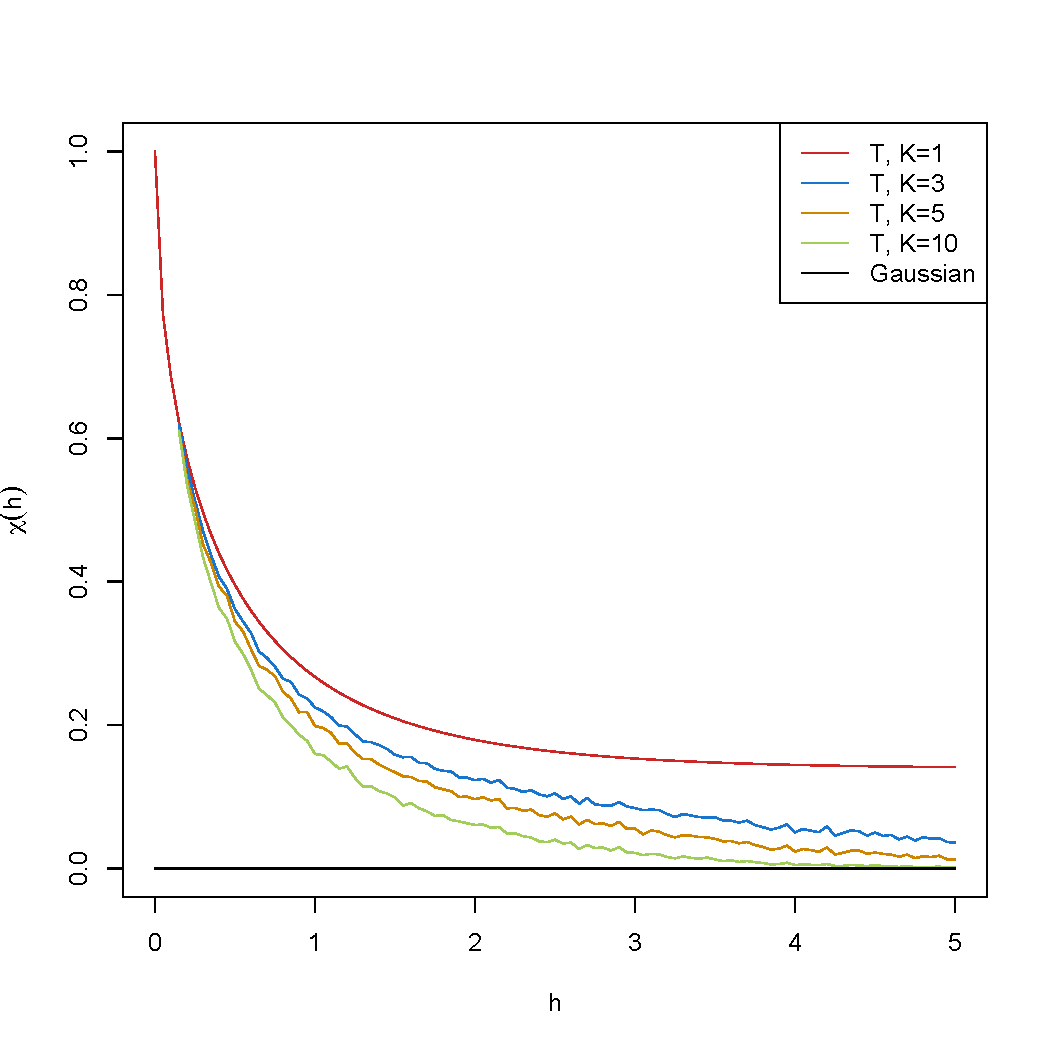
\includegraphics[width=0.5\linewidth]{plots/chi-h.pdf}
  \caption{$\chi(h)$ for $K = 1, 3, 5$, and $10$ partitions as a function of distance.}
  \label{fig:chi}
\end{figure}


\subsection{Extension to space-time data} \label{s:temporal}
When using daily measurements, the assumption of temporal independence is inappropriate.
There are several places where temporal dependence could be incorporated in the model, including the residual $v_t(\bs)$.
However, we choose to allow for temporal dependence in the $\bw$, $z$, and $\sigma$ terms because these terms dictate the tail behavior which is our primary focus.
In this section, we extend (\ref{eq:partition}) to the spatiotemporal setting.
Let
\begin{align} \label{eq:spatiotemp}
  Y_t(\bs) = \bX_t(\bs)^T \bbeta + \lambda \sigma_t(\bs) |z_t(\bs)| + \sigma_t(\bs) v_t(\bs),
\end{align}
where $t \in \{1, \ldots, T\}$ denotes the day of each observation.
Let \hbox{$\bw_{tk} = (w_{tk1}, w_{tk2})$} be a spatial knot on day $t$, and let $w_{t1}, \ldots, w_{tK}$ be a collection of spatial knots on day $t$.
As in section \ref{s:part}, these knots define a daily partition $P_{t1}, \ldots, P_{tK}$, and for $\bs \in P_{tk}$,
\begin{align}
  z_t(\bs) = z_{tk}\\
  \sigma_{t}(\bs) = \sigma_{tk}.
\end{align}

We use an AR(1) time series model for $w_{tk}$, $z_{tk}$, and $\sigma_{tk}$.
The time series model must be specified after a transformation to preserve the skew-$t$ process at each time point.
We first transform the spatial knots from $\calD$ to $\calR^2$ as follows.
Let
\begin{align}
  w^*_{tki} = \Phi^{-1}\left[ \frac{ (w_{tki} - \min(\bs_i))}{ \text{range}(\bs_i) } \right], \quad i = 1, 2
\end{align}
where $\Phi$ is a univariate standard normal density function, and $\bs_i = [s_{1i}, \ldots, s_{ni}]$.
Then $\bw^*_{tk} \in \calR^2$.
We use a copula on the $\sigma^2_t(\bs)$ to ensure that the marginal distributions of $\sigma^2_t(\bs)$ are inverse gamma.
Let
\begin{align}
  \sigma^{2*}_t(\bs) =\Phi^{-1}\left\{ \text{IG}[\sigma^2_t(\bs)] \right\}
\end{align}
where IG is the distribution function for an IG$(a, b)$ random variable.
The AR(1) process for each tail parameter is $\bw^*_{1k} \sim N_w(0, 1)$, $z_{1k} \sim N(0, \sigma^2_{1k})$, $\sigma^{2*}_{1k} \sim N(0, 1)$, and for $t > 1$ the time series is modeled as
\begin{align}
  \bw^*_{tk} | \bw^*_{t-1, k} &\sim N_2\left[\phi_w \bw^*_{t-1, k}, (1 - \phi_w^2) \right] \\
  z_{tk} | z_{t-1, k} &\sim N \left[\phi_z z_{t-1, k}, \sigma^2_{tk} (1 - \phi_z^2)\right] \\
  \sigma^{2*}_{tk} | \sigma^{2*}_{t-1, k} &\sim N \left[\phi_\sigma \sigma^{2*}_{t-1, k}, (1 - \phi_\sigma^2) \right]
\end{align}
where $|\phi_w| < 1$, $0 < \phi_z < 1$, and $|\phi_\sigma| < 1$.
We restrict $\phi_z$ to be positive because in the model, we assume $Y(\bs)$ is a function of $|z_t(\bs)|$.
These are stationary time series models with marginal distributions $\bw^*_{k} \sim N_2(0, 1)$, $z_{k} \sim N(0, \sigma^2_{k})$, $\sigma^{2*}_{k} \sim N(0, 1)$.
After transformation back to the original space, $\bw_{tk} \sim \text{Unif}(\calD)$, $\sigma^2_{tk} \sim \text{IG}(a, b)$.
For each day, the model is identical to the spatial-only model in (\ref{eq:partition}) by construction.

\subsection{Hierarchical model}\label{s:hier}
Conditioned on $z_{tk}(\bs)$, $\sigma^2_{tk}(\bs)$, and $P_{tk}$, the marginal distributions are Gaussian and the joint distribution multivariate Gaussian.
However, we do not fix the partitions, they are treated as unknown and updated in the MCMC.
We model this with a Bayesian hierarchical model as follows.
Let $\bw_{t1}, \ldots, \bw_{tK}$ be a set of daily spatial knots in a spatial domain of interest, $\calD$, and $P_{tk}$ as defined in (\ref{eq:subregions}).

Then
\begin{align}
   Y_t(\bs) \mid z_{t}(\bs), \sigma^2(\bs), P_{tk}, \alpha, \beta, \Theta &= \bX_t(\bs)^T \beta + \lambda |z_t(\bs)| + \sigma_t(\bs) v_t(\bs) \label{eq:hier}\\
   z_t(\bs) &= z_{tk} \text{ if } \bs \in P_{tk}\\
   \sigma^2_{t}(\bs) &= \sigma^2_{tk} \text{ if } \bs \in P_{tk}\\
   \lambda &\sim N(0, 10)\\
   v_t(\bs) \mid \Theta &\sim \Matern(0, \Sigma)\\
   z_{tk} \mid z_{t-1, k}, \sigma^2_{tk} &\sim N(\phi_z z_{t-1, k}, \sigma^2_{tk} (1 - \phi_z^2))\\
   \sigma^{2*}_{tk} \mid \sigma^{2*}_{t-1, k} &\sim N(\phi_\sigma \sigma^{2*}_{t-1, k}, (1 - \phi_\sigma^2))\\
   \bw^*_{tk} \mid \bw^*_{t-1, k} &\sim N_2(\phi_w \bw^*_{t-1, k}, (1 - \phi_w^2))
\end{align}
where $\Theta = \{\rho, \nu, \gamma\}$, and $\Sigma$ is a \Matern covariance matrix as described in Section \ref{s:skewt}.

\section{Computation}\label{s:comp}
First, we impute values below the threshold.
Then, we update $\Theta$ using Metropolis Hastings or Gibbs sampling when appropriate.
Finally, we make spatial predictions using conditional multivariate normal results and the fact that the distribution of $Y_t(\bs) \mid \Theta, z(\bs)$ is the usual multivariate normal distribution with a \Matern spatial covariance structure.

We can use Gibbs sampling to update $Y_t(\bs)$ for censored observations that are below the threshold $T$.
After conditioning on $\lambda$, $z_t(\bs)$ and non-censored observations, $Y_t(\bs)$ has truncated normal full conditionals.
So we sample $Y_t(\bs) \sim N_{(-\infty, T)}(\bX \bbeta, \bSigma)$.
After imputing the censored observations, we update the model parameters.
To update the model parameters, we use standard Gibbs updates for parameters when possible.
In the case Gibbs sampling is not possible, parameters are updated using a random-walk Metropolis Hastings algorithm.
See Appendices A.1 and A.2 for details regarding the MCMC.
The final step of the computation is to use Bayesian Kriging to generate a predictive distribution for $Y_t(\bs^*)$ at prediction location $\bs^*$.
This step is similar to the imputation for censored observations except that the full conditionals are no longer truncated at $T$.

\section{Simulation study}\label{s:simstudy}
In this section, we conduct a simulation study to investigate how the number of partitions and the level of thresholding impact the accuracy of predictions made by the model.

\subsection{Design}\label{s:simdesign}
For all simulation designs, we generate data from the model in Section \ref{s:part} using $n_s=144$ sites and $n_t=50$ independent days.
The sites are generated Uniform$([0, 10] \times [0, 10])$.
We generate data from 6 different simulation designs:
\begin{enumerate} \setlength{\itemsep}{-0.5em}
  \item Gaussian marginal, $K=1$ knot
  \item $T$ marginal, $K=1$ knot
  \item $T$ marginal, $K=5$ knots
  \item Skew-$t$ marginal, $K=1$ knots
  \item Skew-$t$ marginal, $K=5$ knots
  \item Max-stable.
\end{enumerate}
In the first five designs, the $v_t(\bs)$ terms are generated using a \Matern covariance with smoothness parameter $\nu = 0.5$ and spatial range $\rho = 1$.
For the covariance matrices in designs 1 -- 5, the proportion of the variance accounted for by the spatial variation is $\gamma = 0.9$ while the proportion of the variance accounted for by the nugget effect is $0.1$.
In the first design, $\sigma^2 = 2$ is used for all days.
For designs 2 -- 4, $\sigma^2_{tk} \iid \text{IG}(3, 8)$
For designs 1 -- 3, we set $\lambda = 0$.
For designs four and five, $\lambda = 3$ was used, and the $z_t$ are generated as described in (\ref{eq:sitez}).
In the sixth design, we generate from a spatial max-stable distribution \citep{Reich2012}.
In this design, data have marginal distributions that follow a generalized extreme value distribution with parameters $\mu = 1, \sigma=1, \xi=0.2$.
In this model, a random effect is used to induce spatial dependence using 144 spatial knots on a regular lattice in the square $[1, 9] \times [1, 9]$.
For this setting, we set $\gamma = 0.5$.
In all six designs, the mean $\bX \bbeta = 10$ is assumed to be constant across space.

$M = 50$ data sets are generated for each design.
For each data set we fit the data using
\begin{enumerate} \setlength{\itemsep}{-0.5em}
  \item Gaussian marginal, $K=1$ knots
  \item Skew-$t$ marginal, $K=1$ knots, $T=-\infty$
  \item Skew-$t$ marginal, $K=1$ knots, $T=q(0.80)$
  \item Skew-$t$ marginal, $K=5$ knots, $T=-\infty$
  \item Skew-$t$ marginal, $K=5$ knots, $T=q(0.80)$
\end{enumerate}
where $q(0.80)$ is the 80th sample quantile of the data.
The design matrix $\bX$ includes an the intercept with a prior of $\beta \sim \text{N}(0, 10)$.
The spatial covariance parameters have priors $\log(\nu) \sim \text{N}(-1.2, 1)$, $\gamma \sim \text{U}(0, 1)$, $\log(\rho) \sim \text{N}(-2, 1)$.
The skewness parameter has prior $\lambda \sim \text{N}(0, 2)$.
The residual variance terms have priors $\sigma^2_t(\bs) \sim \text{IG}(0.1, 0.1)$.
The knots have priors $\bw \sim \text{Unif}(\calD)$.
We do not fit the data using the max-stable methods from \citet{Reich2012} because of the time it takes.

\subsection{Cross validation}\label{s:modelselect}
Models were compared using cross validation with 100 sites used as training sites and 44 sites witheld for testing.
The model was fit using the training set, and predictions were generated at the testing site locations.
Because one of the primary goals of this model is to predict extreme events, we use Brier scores to select the model that best fits the data \citep{Gneiting2007}.
The Brier score for predicting exceedance of a threshold $c$ is given by $[e(c) - P(c)]^2$ where $e(c) = I[y>c]$ is an indicator function indicating that a test set value, $y$, has exceeded the threshold, $c$, and $P(c)$ is the predicted probability of exceeding $c$.
We average the Brier scores over all test sites and days.
For the Brier score, a lower score indicates a better fit.

\subsection{Results}\label{s:simresults}
We compared the Brier scores for exceeding 11 different thresholds for each dataset.
The thresholds used for the Brier scores are extreme quantiles from the simulated data.
Figure \ref{fig:simbrierscores} gives the Brier score relative to the Brier score for the Gaussian method calculated as
\begin{align*}
  \text{BS}_{\text{rel}} = \frac{\text{BS}_{\text{method}}}{\text{BS}_{\text{Gaussian}}}.
\end{align*}
We analyzed the results for the simulation study using two-sided Wilcoxon signed rank tests.
For the first five data settings, our model with no thresholding and $K = 1$ or $5$ partitions performs significantly better (p-value $<0.001$) than the Gaussian method.
Additionally, for the $T$ and skew-$t$ settings with $K = 5$, the skew-$t$ method with $K=5$ partitions performs significantly better (p-value $<0.001$) than the skew-$t$ method with $K=1$ partition except for the Brier score at $T = q(0.995)$ for the $T$ setting with $K = 5$ (p-value $=0.036$).
For the $T$ and skew-$t$ settings with $K = 1$, the Brier scores for the model with $K = 1$ partition are significantly better (p-value $<0.001$) for thesholds less than $q(0.95)$.
However, as the threshold for the Brier score increases, the difference becomes less significant.
Finally, in the max-stable data setting, our model with $K=1$ partition has significantly better Brier scores than the Gaussian method for thresholds $q(0.92)$ -- $q(0.95)$ (p-value $<0.05$) and $q(0.95)$ -- $q(0.995)$ (p-value $<0.001$).

\begin{figure}
  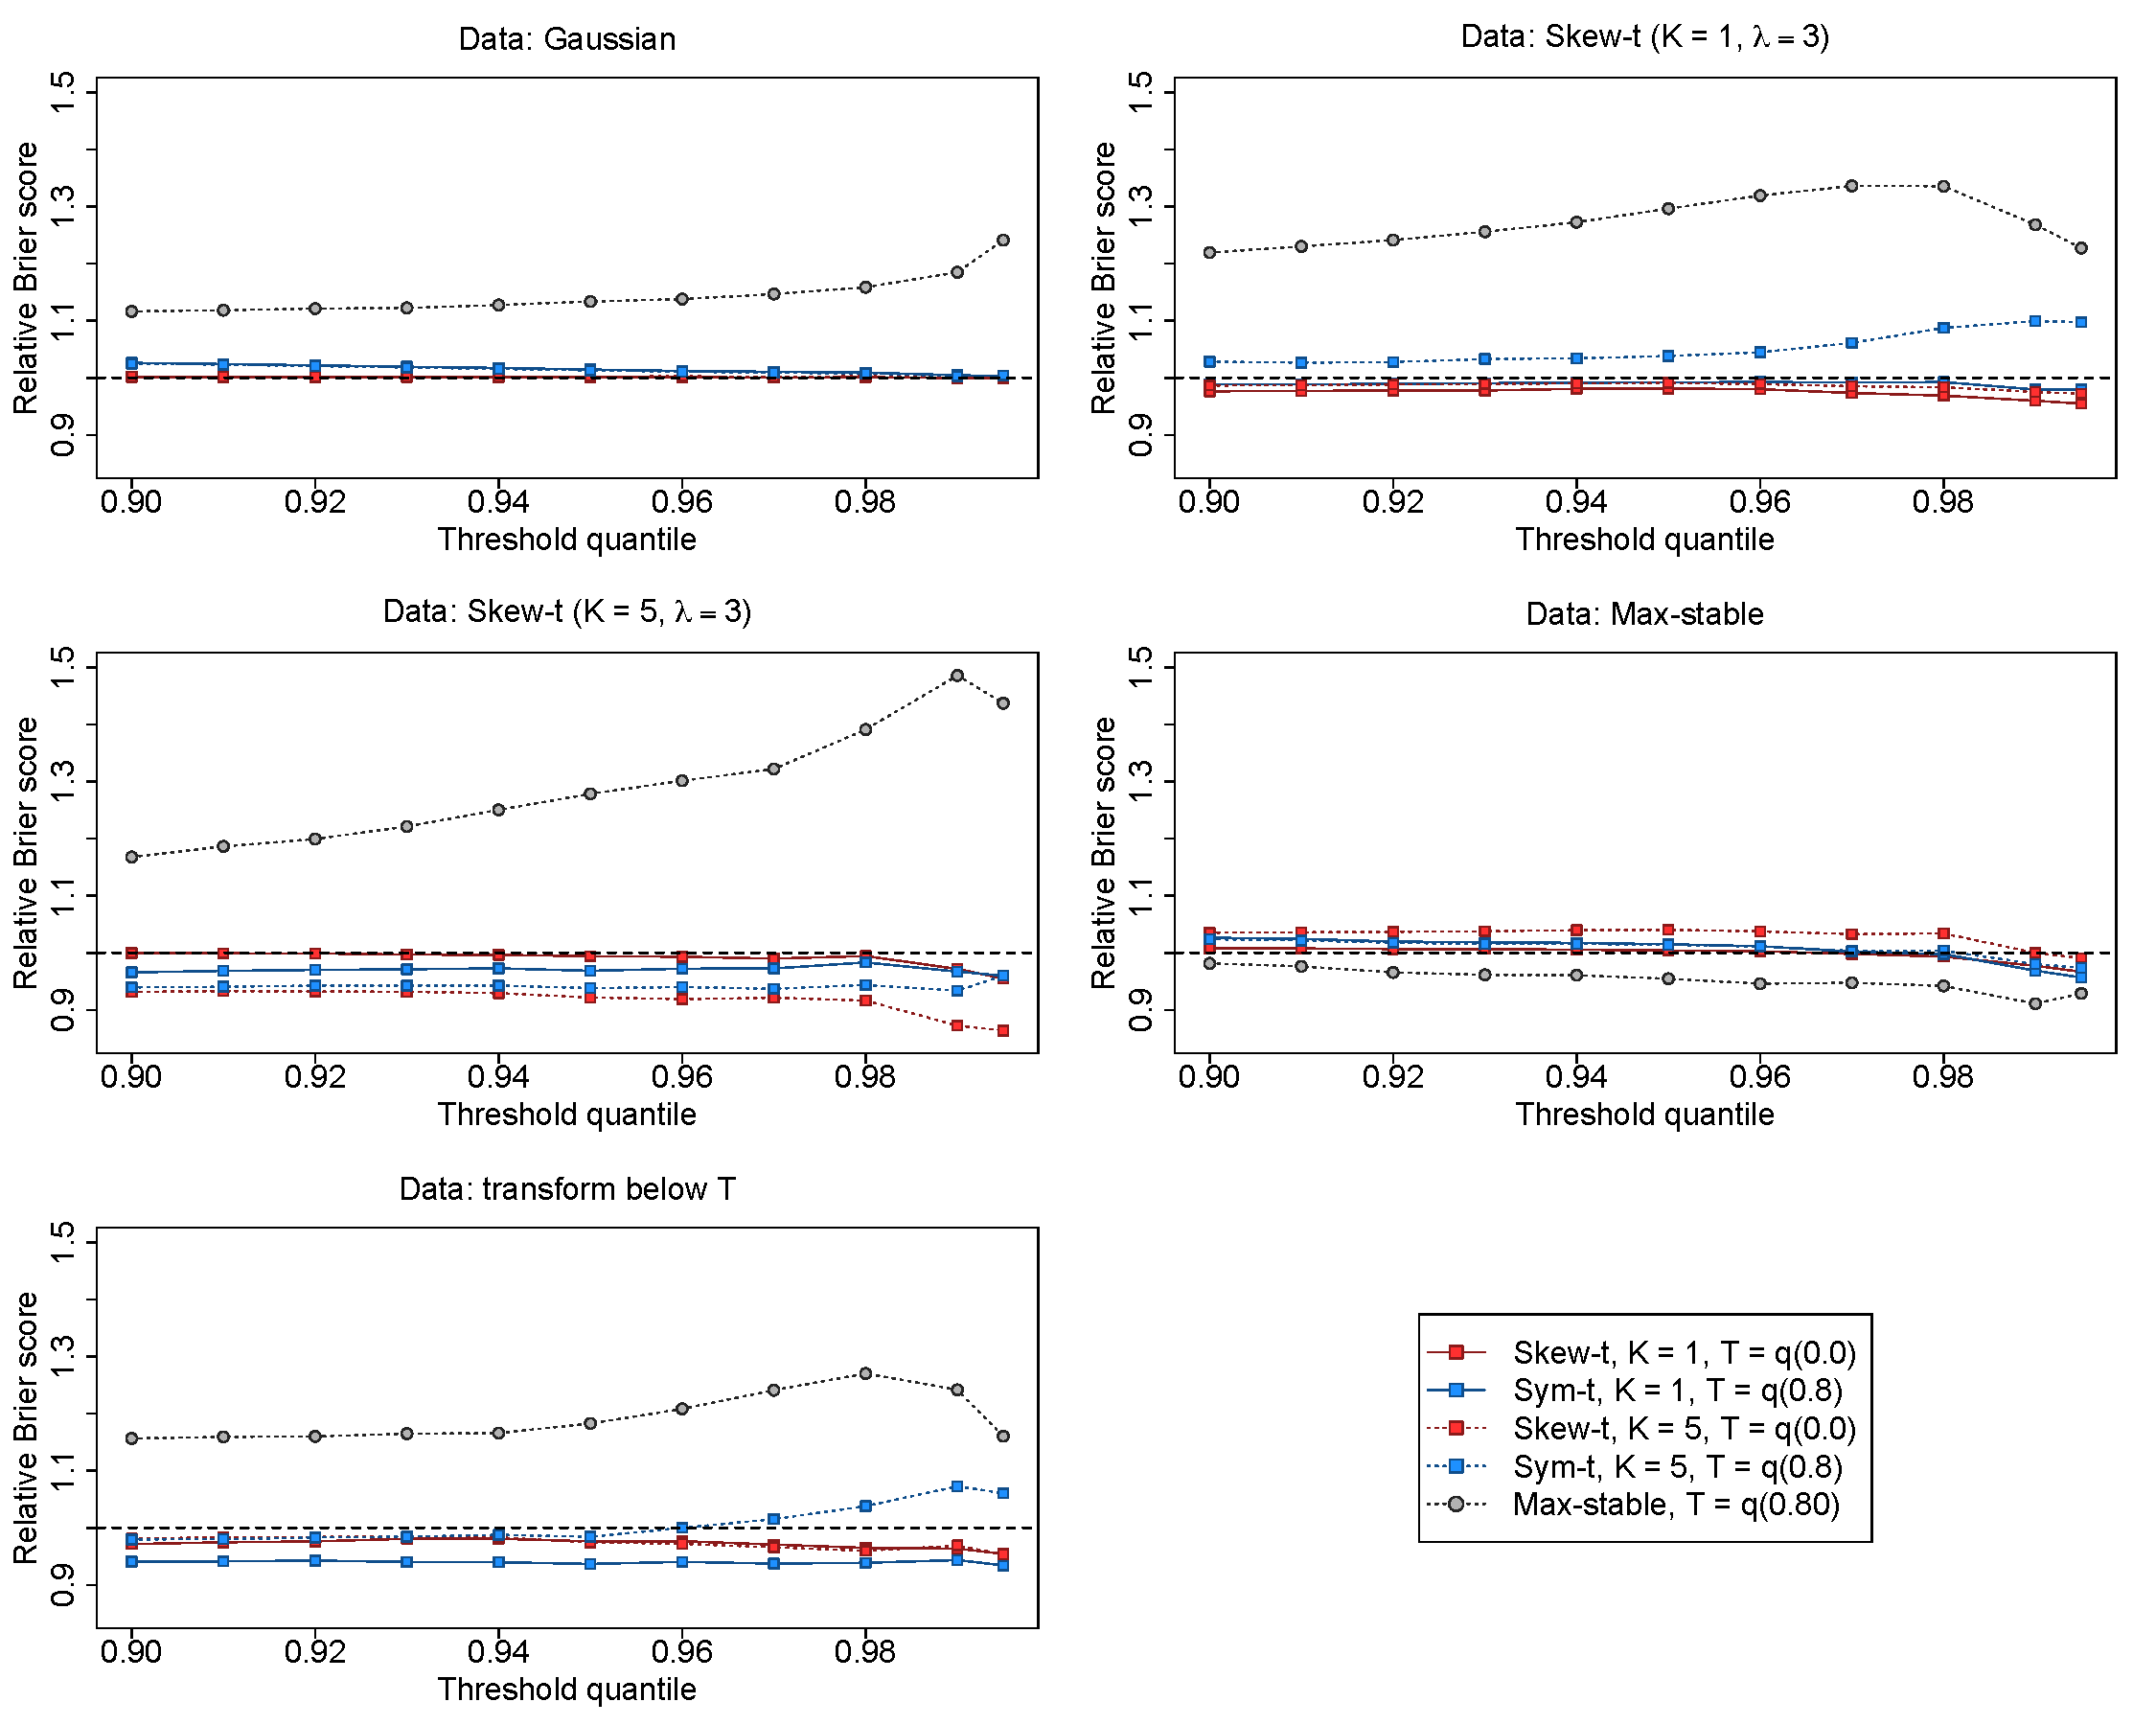
\includegraphics[width=\linewidth]{plots/bsplots-mean.pdf}
  \caption{Brier scores relative to the Gaussian method for simulation study results. A ratio lower than 1 indicates that the method outperforms relative to the Gaussian method.}
  \label{fig:simbrierscores}
\end{figure}

\section{Data analysis}\label{s:analysis}
To illustrate this method, we consider the daily maximum 8-hour ozone measurements for July 2005 at 735 Air Quality System (AQS) monitoring sites in the eastern United States as the response (see Figure \ref{fig:ozone}).
For each site, we also have covariate information containing the estimated ozone from the Community Multi-scale Air Quality (CMAQ) modeling system.
Initially, we fit a linear regression assuming a mean function of
\begin{align}
  \bX \bbeta = \beta_0 + \beta_1 \cdot \text{CMAQ}_t(\bs). \label{eq:datamean}
\end{align}
The data from July 10 are shown in Figure \ref{fig:ozone} along with a Q-Q plot of the residuals compared to a skew-$t$ distribution with 10 d.f. and $\alpha = 1$.
\begin{figure}
  \centering
  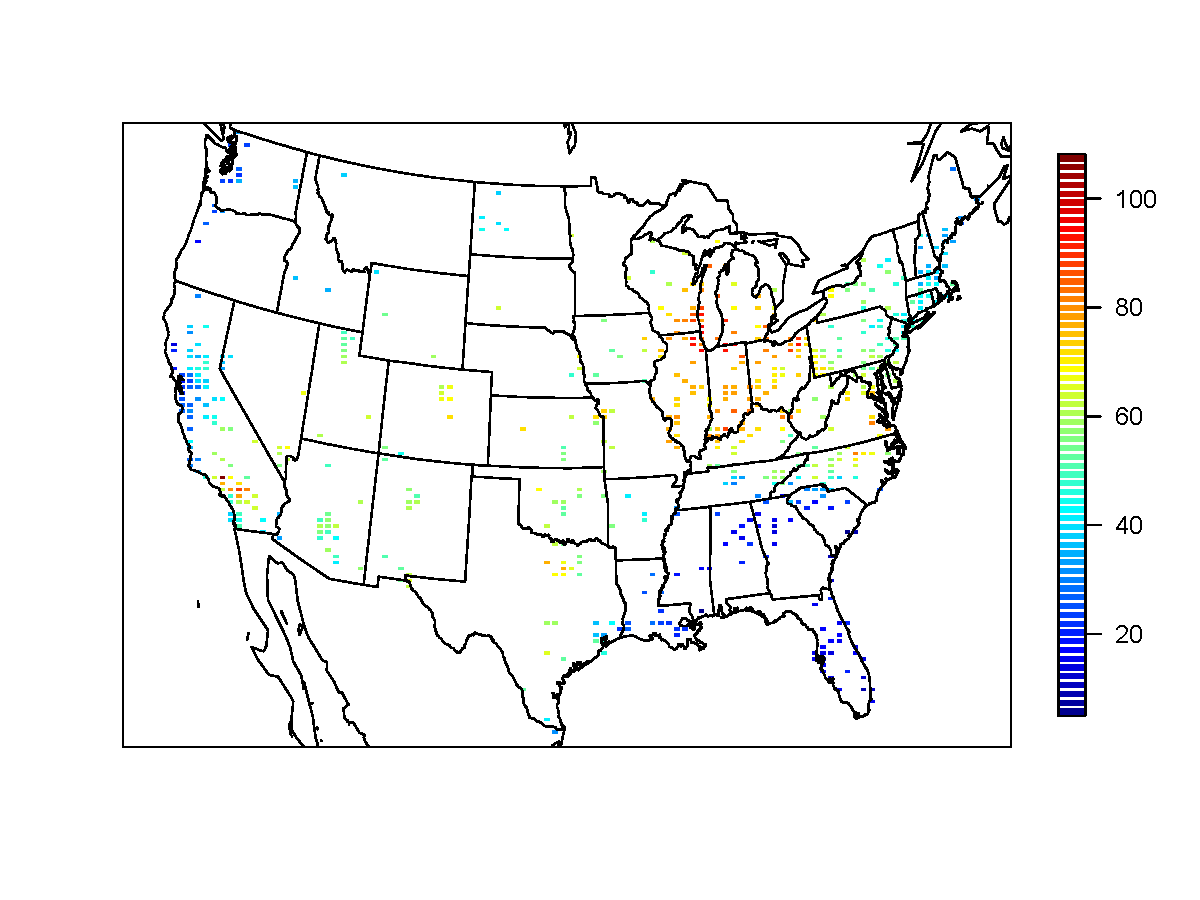
\includegraphics[width=0.55\linewidth]{plots/ozone-10jul-us.pdf}
  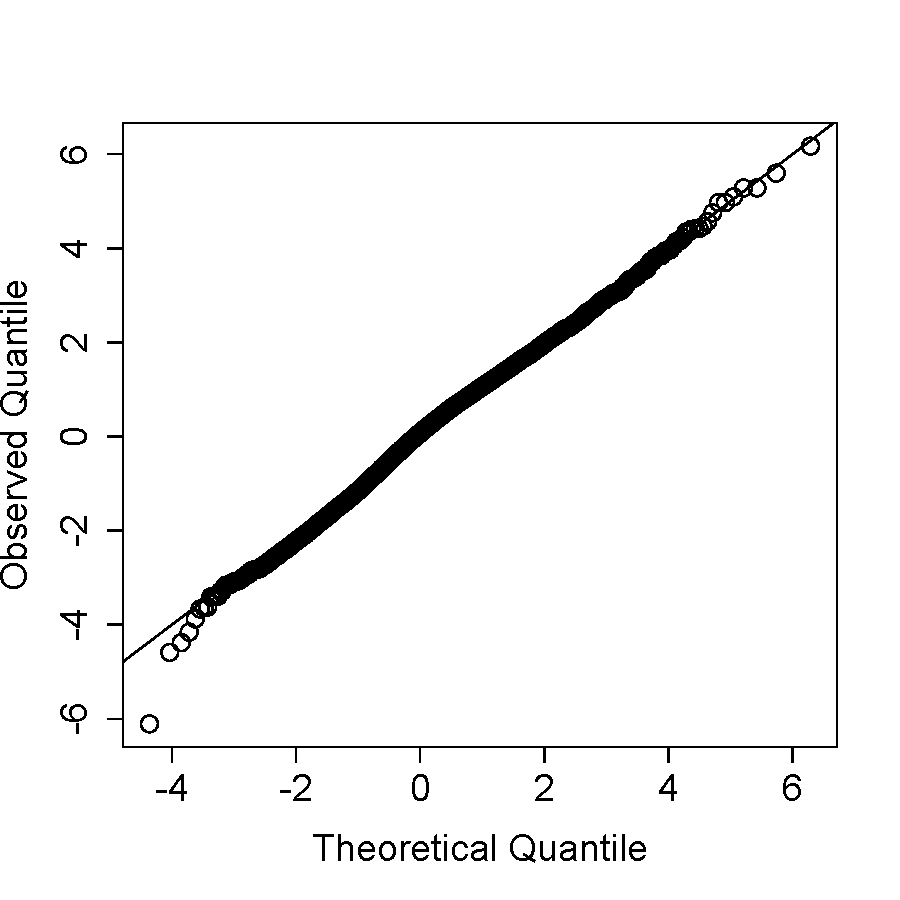
\includegraphics[width=0.44\linewidth]{plots/qq-res.pdf}
  \caption{Ozone values on 10 July 2005 (left) Q-Q plot of the residuals (right)}
  \label{fig:ozone}
\end{figure}

We explore spatial and temporal extremal dependence by considering $\chi_c = \Pr[Y(\bs) > c | Y(\bt) > c]$.
To examine spatial dependence in high quantiles, we consider observations at all pairs of sites $\bs$ and $\bt$ that are distance $h$ apart where $h$ is separated into bins of size 0.25 km.
Then conditioned on $Y(\bt) > c$, we take the sample proportion of $Y(\bs) > c$.
Finally, $\widehat{\chi}_c(h)$ is averaged over all days at each of the three threshold quantiles.
To examine temporal dependence in high quantiles, we consider observations at a single site that are taken lag-$t$ days apart.
Then conditioned on $Y_n(\bs) > c$, we take the sample proportion of $Y_{n + t}(\bs) > c$.
Finally, $\widehat{\chi}(t)$ is averaged over all sites at each of the three threshold quantiles.
The $\widehat{\chi}_c(h)$ and $\widehat{\chi}_c(t)$ plots in Figure \ref{fig:chi-st} show the estimated spatial and temporal dependence of the residuals for the ozone data at three quantile levels $q(0.90), q(0.95)$, and $q(0.99)$.
Both plots indicate that there is dependence in the high quantile levels beyond what we expect if the residuals were independent.
\begin{figure}
  \centering
  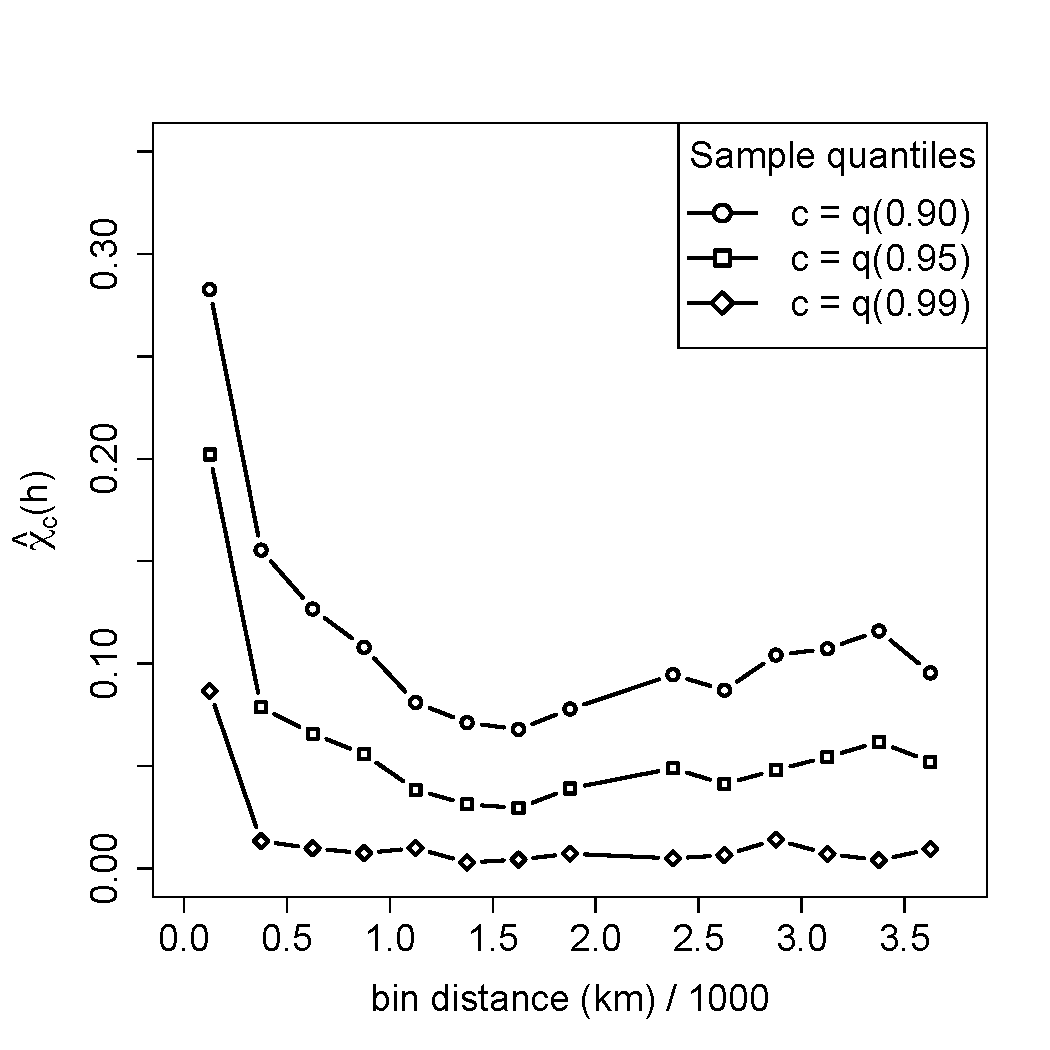
\includegraphics[width=0.49\linewidth]{plots/chi-h-ozone.pdf}
  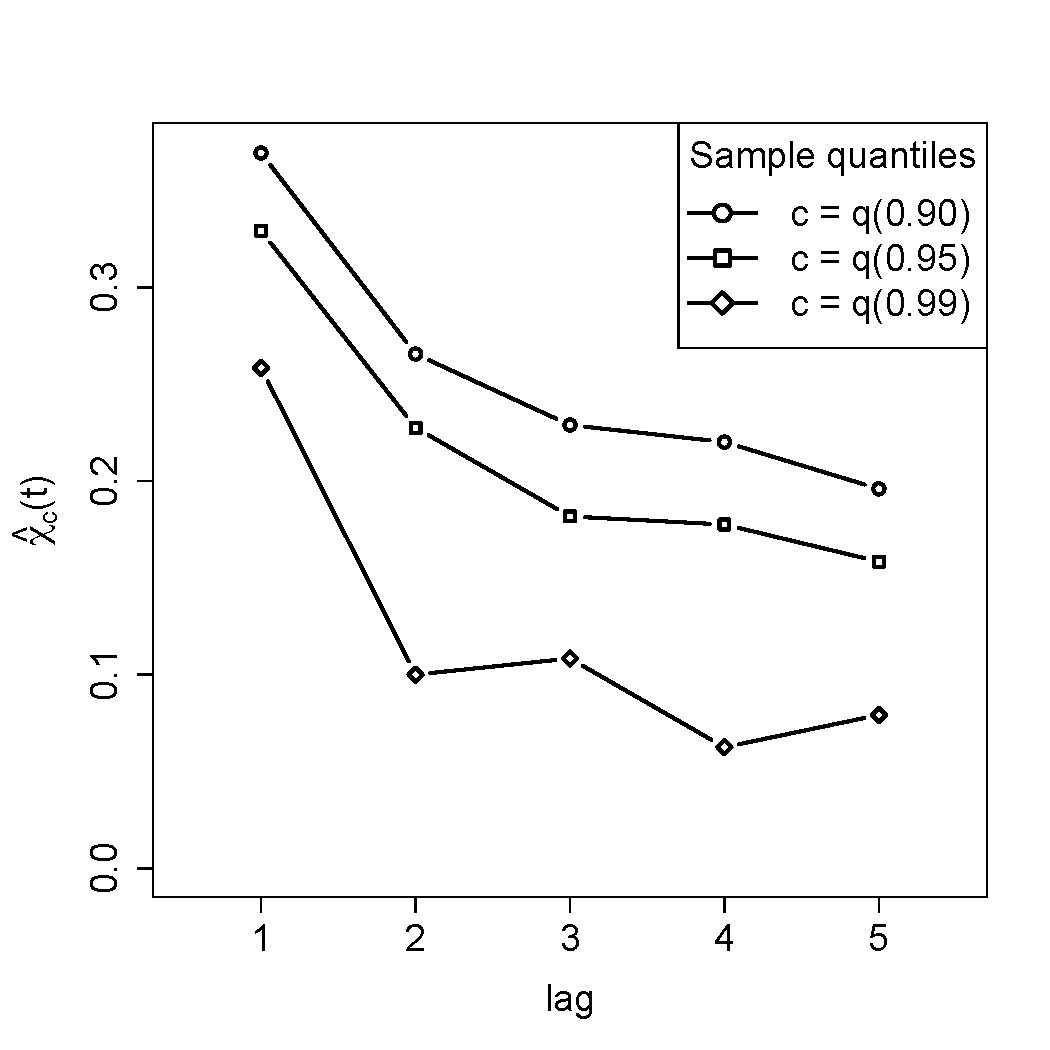
\includegraphics[width=0.49\linewidth]{plots/chi-t-ozone.pdf}
  \caption{$\widehat{\chi}_c(h)$ plot for the residuals (left). $\widehat{\chi}_c(t)$ plot for the residuals (right).}
  \label{fig:chi-st}
\end{figure}

\subsection{Model comparisons}
The data analysis was done in two stages.
In the first stage, we fit the model using Gaussian and skew-$t$ marginal distributions with $K=1, 5, 10, 15$ partitions.
We chose to censor $Y(\bs)$ at $T = 0, 50, 75, 85$ ppb in order to compare results from no, moderate, and high censoring.
We also include a max-stable analysis using the hierarchical max-stable model of \citet{Reich2012}.
All methods assume the mean function given in (\ref{eq:datamean}).
For each model, Brier scores were were averaged over all sites and days to obtain a single Brier score for each dataset.
At a particular threshold or quantile level, the model that fits the best is the one with the lowest score.
Based on the results from the first stage, we conducted a second stage analysis with $K = 6, 7, 8, 9$.

\subsection{Results}\label{s:results}
The plot in Figure \ref{fig:bs-ozone} shows the relative Brier scores (see Section \ref{s:simresults}) for the first and second stages of the analysis.
\begin{figure}
  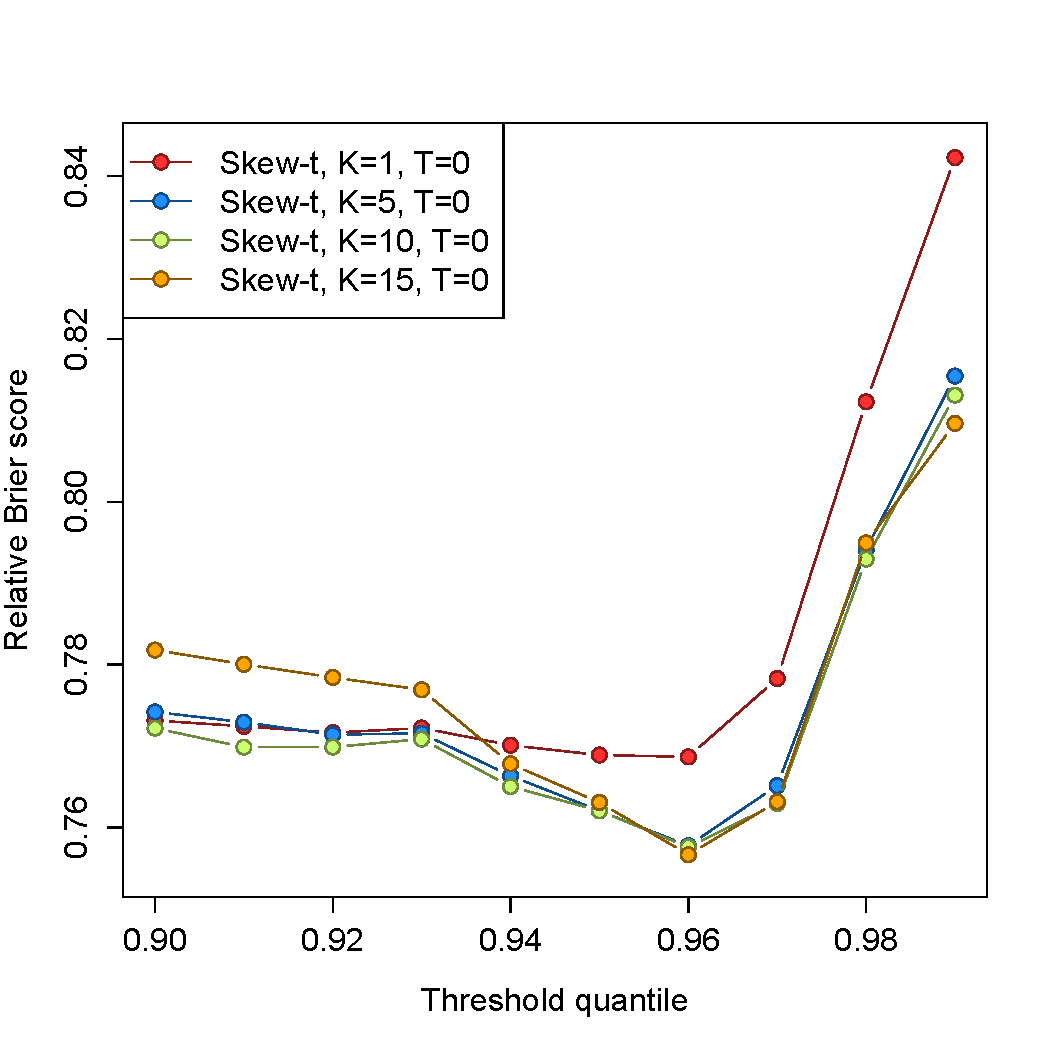
\includegraphics[width=0.5\linewidth]{plots/bs-ozone-1.pdf}
  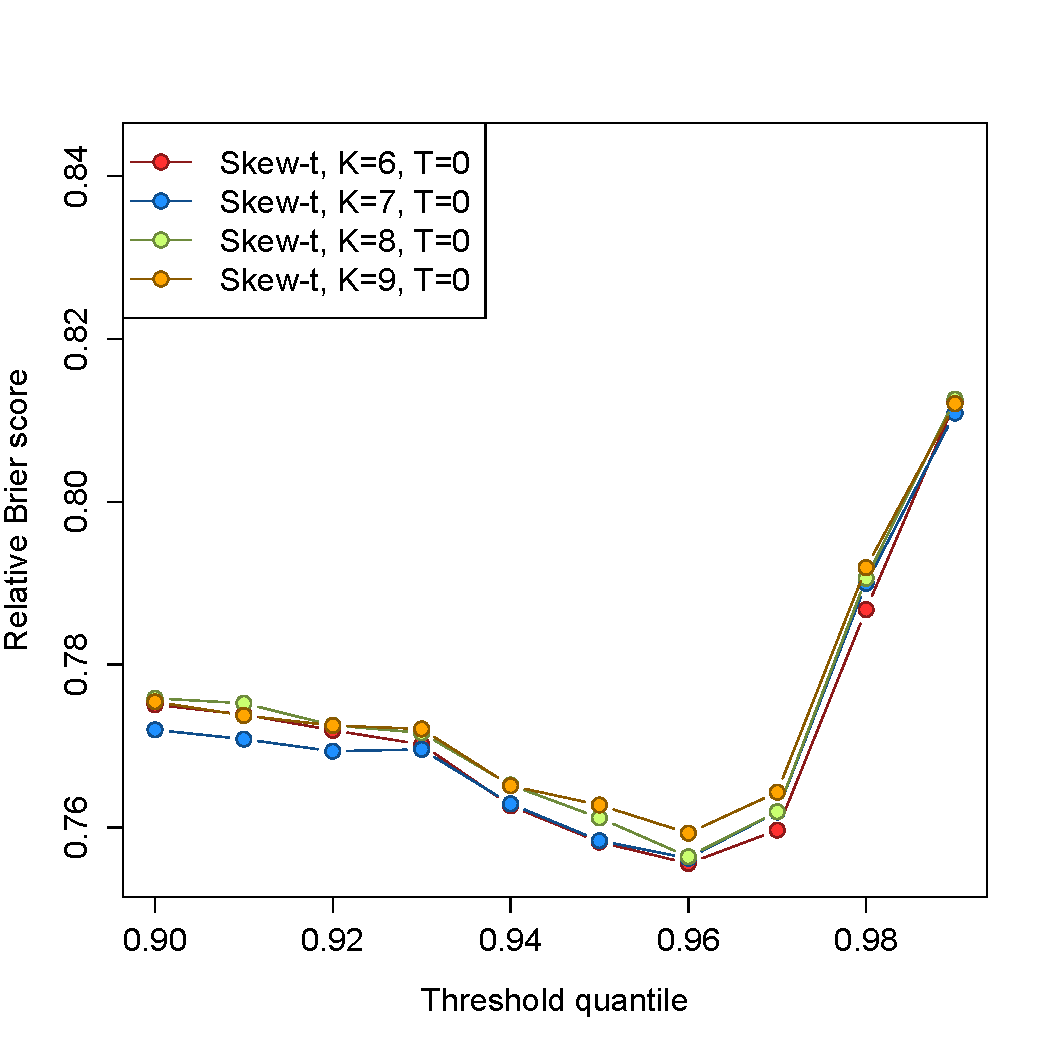
\includegraphics[width=0.5\linewidth]{plots/bs-ozone-2.pdf}
  \caption{Relative Brier scores for stage 1 ozone analysis (left) and stage 2 ozone analysis (right)}
  \label{fig:bs-ozone}
\end{figure}
As with the simulation results, the Brier scores from the thresholded models were higher than those from the non-thresholded models, so we do not include them here.
Based upon these results, it would appear that our model using a partition with anywhere from $K = 5$ to $K = 10$ partitions gives Brier scores across all threshold levels that are consistently low.

\section{Discussion}\label{s:con}
In this paper we propose a new approach for spatitemporal modeling of extreme values.
The proposed model gives flexible tail behavior, demonstrates asymptotic dependence for observations at sites that are near to one another, and has computation on the order of Gaussian models for large space-time datasets.
In the simulation study, we demonstrate that there are statistically significant improvements over a na\"{i}ve Gaussian approach.
In both the simulation study, and the application to ozone data, we find that incorporating a partition in the model improves extreme prediction.
We also find that censoring the data below a threshold does not improve the results, and in many cases makes them worse.

This model presents new avenues for future research.
One possibility is the implementation of a different partition structure.
We choose to define the random effects for a site by using an indicator function based on closeness to a knot.
However, this indicator function could be replaced by kernel function that would allow for multiple knots to impact each site, with the weight of each knot to be determined by some characteristic such as distance.
Another area that should be explored is the temporal dependence in the model.
Instead of implementing a time series on the random effects, a three-dimensional covariance structure on the residuals could be implemented to address temporal dependence.

\section*{Acknowledgments}

\appendix
\section{Appendices}
\subsection{MCMC details} \label{a:mcmc}
The MCMC sampling for the model \ref{s:hier} is done using {\tt R} (http://www.r-project.org). Whenever possible, we select conjugate priors (see Appendix \ref{a:posterior}); however, for some of the parameters, no conjugate prior distributions exist.
When no conjugate prior distribution exists, we use a random walk Metropolis Hastings update step.
In each Metropolis Hastings update, we tune the algorithm to give acceptance rates near 0.40.

\subsubsection*{Spatial knot locations}
For each day, we update the spatial knot locations, $\bw_1, \ldots, \bw_K$, using a Metropolis Hastings block update.
Because the spatial domain is bounded, we generate candidate knots using the transformed knots $\bw^*_1, \ldots, \bw^*_K$ (see section \ref{s:temporal}) and a random walk bivariate Gaussian candidate distribution
\begin{align*}
	{\bw^*_k}^{(c)} \sim \text{N}({\bw^*_k}^{(r - 1)}, s^2 I_2)
\end{align*}
where ${\bw^*_k}^{(r - 1)}$ is the location for the transformed knot at MCMC iteration $r - 1$, $s$ is a tuning parameter, and $I_2$ is an identity matrix.
After candidates have been generated for all $K$ knots, the acceptance ratio is
\begin{align*}
  R = \left\{ \frac{ l[ Y_t(\bs | \bw_1^{(c)}, \ldots, \bw_K^{(c)}, \ldots)] }{l[ Y_t(\bs | \bw_1^{(r - 1)}, \ldots, \bw_K^{(r - 1)}, \ldots)]} \right\} \times \left\{ \frac{ \prod_{k = 1}^{K}\phi(\bw_k^{(c)})}{ \prod_{k = 1}^{K}\phi(\bw_k^{(r - 1)})} \right\} \times \left\{ \frac{ \prod_{k = 1}^{K} p({\bw^*_k}^{(c)})}{ \prod_{k = 1}^{K} p({\bw^*_k}^{(r - 1)})}\right\}
\end{align*}
where $l$ is the likelihood given in (\ref{eq:hier}), and $p(\cdot)$ is the prior either taken from the time series given in (\ref{s:temporal}) or assumed to be uniform over $\calD$.
The candidate knots are accepted with probability $\min\{R, 1\}$.

\subsubsection*{Spatial random effects}
If there is temporal dependence amongst the observations, then we update $z_{tk}$ using a Metropolis Hastings update.
First, we generate a candidate using a random walk Gaussian candidate distribution
\begin{align*}
  z_{tk}^{(c)} \sim \text{N}(z_{tk}^{(r - 1)}, s^2)
\end{align*}
where $z_{tk}^{(r-1)}$ is the value at MCMC iteration $r - 1$, and $s$ is a tuning parameter.
The acceptance ratio is
\begin{align*}
  R = \left\{ \frac{ l[Y_t(\bs) | z_{tk}^{(c)}, \ldots] }{ l[Y_t(\bs) | z_{tk}^{(r - 1)}]} \right\} \times \left\{ \frac{ p[ z_{tk}^{(c)} ] }{ p[ z_{tk}^{(r - 1)}]}\right\}.
\end{align*}
The candidate is accepted with probability $\min\{R, 1\}$.

\subsubsection*{Variance terms}
When there is more than one site in a partition, then we update $\sigma^2_{tk}$ using a Metropolis Hastings update.
First, we generate a candidate for $\sigma^2_{tk}$ using an IG$(a^*/s, b^*/s)$ candidate distribution in an independence Metropolis Hastings update where $a^* = (n_{tk} + 1) / 2 + a$, $b^* = [Y_{tk}^T \Sigma^{-1}_{tk} Y_{tk} + z_{tk}^2] / 2 + b$, $n_{tk}$ is the number of sites in partition $k$ on day $t$, and $Y_{tk}$ and $\Sigma^{-1}_{tk}$ are the observations and precision matrix for partition $k$ on day $t$.
The acceptance ratio is
\begin{align*}
  R = \left\{
    \frac{ l[Y_t(\bs) | {\sigma^2_{tk}}^{(c)}, \ldots] }
         { l[Y_t(\bs) | {\sigma^2_{tk}}^{(r - 1)}]}
    \right\} \times \left\{
    \frac{ l[z_{tk} | {\sigma^2_{tk}}^{(c)}, \ldots] }
         { l[z_{tk} | {\sigma^2_{tk}}^{(r - 1)}, \ldots] }
    \right\} \times \left\{
    \frac{ p[ {\sigma^2_{tk}}^{(c)} ] }
         { p[ {\sigma^2_{tk}}^{(r - 1)}] }
    \right\} \times \left\{
    \frac{ c[ {\sigma^2_{tk}}^{(r - 1)}] }
         { c[ {\sigma^2_{tk}}^{(c)}]}
    \right\}
\end{align*}
where $p[\cdot]$ is the prior either taken from the time series given in (\ref{s:temporal}) or assumed to be IG$(a, b)$, and $c[\cdot]$ is the candidate distribution.
The candidate is accepted with probability $\min\{R, 1\}$.

\subsubsection*{Spatial covariance parameters}
We update the three spatial covariance parameters, $\log(\rho)$, $\log(\nu)$, $\gamma$, using a Metropolis Hastings block update step.
First, we generate a candidate using a random walk Gaussian candidate distribution
\begin{align*}
	\log(\rho)^{(c)} \sim \text{N}(\log(\rho)^{(r - 1)}, s^2)
\end{align*}
where $\log(\rho)^{(r-1)}$ is the value at MCMC iteration $r - 1$, and $s$ is a tuning parameter.
Candidates are generated for $\log(\nu)$ and $\gamma$ in a similar fashion.
The acceptance ratio is
\begin{align*}
	R = \left\{ \frac{ \prod_{t = 1}^{T} l[Y_t(\bs) | \rho^{(c)}, \nu^{(c)}, \gamma^{(c)}, \ldots] }{\prod_{t = 1}^{T} l[Y_t(\bs) | \rho^{(r-1)}, \nu^{(r-1)}, \gamma^{(r-1)}, \ldots] } \right\} \times \left\{ \frac{ p[\rho^{(c)}] }{ p[\rho^{(r - 1)] } } \right\} \times \left\{ \frac{ p[\nu^{(c)}] }{ p[\nu^{(r - 1)}] } \right\} \times \left\{ \frac{ p[ \gamma^{(c)} ] }{ p[\gamma^{(r - 1)} ] } \right\}.
\end{align*}
All three candidates are accepted with probability $\min\{R, 1\}$.

\subsection{Posterior distributions} \label{a:posterior}



%\subsubsection*{Conditional posterior of $U | Y$}\label{s:condu}
% Let $Y_i | U \sim \mbox{N}(U, \sigma^2)$, $i = 1, \ldots, n$, let $\tau = 1 / \sigma^2$, and let $\pi(U) \propto \exp \left\{ -\frac{ u^2 \theta }{ 2 } \right\}$. 
% Then the conditional posterior of $U \mid \ldots$ is 
% \begin{align}
%   \pi (U \mid \ldots) & \propto \exp \left\{ -\frac{ u^2 \theta }{ 2 } \right\} \exp \left\{ - \sum_{i = 1 }^n\frac{ \tau (y_i - u)^2 }{ 2 } \right\} \nonumber \\
%     & \propto \exp \left\{ -\frac{ 1 }{ 2 } \left[ u^2 \theta + \sum_{i=1 }^n\tau (y_i^2 - 2y_iu + u^2) \right] \right\} \nonumber \\
%     & \propto \exp \left\{ - \frac{ 1 }{ 2 }\left( u - \frac{ \tau \sum_{i=1}^n y_i }{ \theta + n \tau } \right)^2 \left( \theta + n \tau \right) \right\} \nonumber\\
%     & \propto \mbox{HN}(\xi^*, \theta^*) \label{eq:condu}
% \end{align}
% where 
% \begin{align*}
%   \xi^* &= \frac{ \tau \sum_{i=1}^n y_i }{ \theta + n \tau }\\
%   \theta^* &= \theta + n \tauå
% \end{align*}

\subsubsection*{Conditional posterior of $z_{tl} \mid \ldots $}\label{s:mvcondu}
For simplicity, drop the subscript $t$ and define 
\begin{align*}
R(\bs) = \left\{ 
    \begin{array}{ll}
        Y(\bs) - X(\bs) \beta &s \in P_l\\[1em]
        Y(\bs) - X(\bs) \beta - \delta z(\bs) \qquad & s \notin P_l
    \end{array} 
\right.
\end{align*}
Let 
\begin{align*}
    R_1 &= \text{the vector of } R(\bs) \text{ for } s \in P_l \\
    R_2 &= \text{the vector of } R(\bs) \text{ for } s \notin P_l \\
    \Omega &= \Sigma^{-1}.
\end{align*}
Then
\begin{align*}
    \pi(z_l | \ldots) &\propto \exp \left\{ -\frac{ 1 }{ 2 \sigma^2 } \left[ \frac{ 1 }{ (1 - \delta^2)}
        \left( \begin{array}{c}
            R_1 - \delta z_l \bOne\\
            R_2
        \end{array} \right)^T
        \left( \begin{array}{cc}
            \Omega_{11} & \Omega_{12}\\
            \Omega_{21} & \Omega_{22}
        \end{array} \right)
        \left( \begin{array}{c}
            R_1 - \delta z_l \bOne\\
            R_2
        \end{array} \right)
        +  z_l^2 \right]
    \right\} I(z_l > 0) \\
        &\propto \exp \left\{ -\frac{ 1 }{ 2 \sigma^2 } \left[ \Lambda_z z_l^2 - 2 \mu_z z_l \right] \right\} I(z_l > 0)
\end{align*}
where
\begin{align*}
    \mu_z &= \frac{ \delta}{(1 - \delta^2)} ( R_1^T \Omega_{11} + R_2^T \Omega_{21} )\bOne\\
    \Lambda_z &= \frac{\delta^2 \bOne^T \Omega_{11} \bOne }{ (1 - \delta^2) } + 1.
\end{align*}
Then $Z_l | \ldots \sim N_{(0, \infty)} (\Lambda_z^{-1} \mu_z, \sigma^2 \Lambda_z^{-1})$
\subsection*{Conditional posterior of $\beta \mid \ldots$}\label{s:betapost}
Let $\beta \sim \mbox{N}_{p}(0, \Lambda_0)$ where $\Lambda_0$ is a precision matrix. Then 
\begin{align*}
    \pi(\beta \mid \ldots) & \propto \exp \left\{ - \frac{ 1 }{ 2 } \beta^T \Lambda_0 \beta - \sum_{t = 1 }^T \frac{ 1 }{ 2 } [\bY_t(\bs) - X_t(\bs) \beta - \sigma \delta |u_t|]^T \Sigma^{-1} [\bY_t(\bs) - X_t(\bs) \beta - u^*_t] \right\}\\
     & \propto \exp \left\{ -\frac{ 1 }{ 2 } \left[ \beta^T \Lambda_p \beta  - \sum_{ t = 1 }^T 2 [ \beta^T X_t(\bs) \Sigma^{-1} (\bY_t(\bs) + u^*_t )] \right] \right\}\\
     & \propto \mbox{N}_p ( \mu_p , \Lambda_p)
\end{align*}
where
\begin{align*}
    \mu_p &= \Lambda_p^{-1} \left[ X_t(\bs)^T \Sigma^{-1} (\bY_t(\bs) + u^*_t) \right]\\
    \Lambda_p &= \left (\Lambda_0 + \sum_{ t = 1 }^{ T} X_t(\bs)^T \Sigma^{-1} X_t(\bs) \right)
\end{align*}
and $\Lambda_p$ is a precision matrix.
\subsection*{Conditional posterior of $\sigma^2 \mid \ldots$}\label{s:sigpost}
In the case where $L = 1$, then $\sigma^2$ has a conjugate posterior distribution. 
Let $\sigma_t^2 \iid \mbox{IG}(\alpha_0, \beta_0)$. For simplicity, drop the subscript $t$. Then
\begin{align*}
    \pi(\sigma^2 \mid \ldots) & \propto (\sigma^2)^{ -\alpha_0 - 1 / 2 - n / 2 - 1} \exp \left\{ -\frac{\beta_0}{\sigma^2} - \frac{ z^2 }{2 \sigma^2} - \frac{ (\bY - \bmu)^T \Sigma^{-1} (\bY - \bmu) }{2 \sigma^2} \right\} \\
    & \propto (\sigma^2)^{ -\alpha_0 - 1 / 2 - n / 2 - 1} \exp \left\{ - \frac{ 1 }{ \sigma^2 } \left[\beta_0 + \frac{ z^2 }{ 2 } + \frac{ 1 }{ 2 } (\bY - \bmu)^T \Sigma^{-1} (\bY - \mu) \right] \right\} \\
    & \propto \mbox{IG} (\alpha^*, \beta^*)
\end{align*}
where
\begin{align*}
    \alpha^* &= \alpha_0 + \frac{1}{2} + \frac{n}{2} \\
    \beta^* &= \beta_0 + \frac{ z^2 }{ 2 } + \frac{ 1 }{ 2 }(\bY - \bmu)^T \Sigma^{-1} (\bY - \bmu).
\end{align*}
In the case that $L > 1$, a random walk Metropolis Hastings step will be used to update $\sigma^2_{lt}$.
\subsection*{Conditional posterior of $\lambda \mid \ldots$}\label{s:lambdapost}
Let $\lambda \sim N(0, \tau_\lambda)$ where $\tau_\lambda$ is a precision term. Then
\begin{align*}
  \pi(\lambda \mid \ldots) &\propto \exp \left\{ -\frac{ 1 }{ 2 } \tau_\lambda \lambda^2 + \sum_{ t = 1 }^T \frac{ 1 }{ 2 } [\bY_t - X_t\beta - \lambda |z_t|]^T \Omega [\bY_t - X_t\beta - \lambda |z_t|] \right\} \\
      &\propto \exp \left\{ -\frac{ 1 }{ 2 } [\lambda^2(\tau_\lambda + \sum_{t = 1 }^T |z_t|^T \Omega |z_t|^T) - 2 \lambda \sum_{t=1}^T[|z_t|^T \Omega (\bY_t - X_t \beta) \right\}\\
      &\propto \exp \left\{ -\frac{ 1 }{ 2 } [\tau_\lambda^* \lambda^2 - 2 \mu_\lambda] \right\}
\end{align*}
where
\begin{align*}
  \mu_\lambda &= \sum_{t = 1}^T |z_t|^T \Omega (\bY_t - X_t \beta)\\
  \tau_\lambda^* &= t_\alpha + \sum_{t=1}^T |z_t|^T \Omega |z_t|.
\end{align*}
Then $\lambda \mid \ldots \sim N(\tau^{*-1}_\lambda \mu_\lambda, \tau^{*-1}_\lambda) $

\subsection{Proof that $\lim_{h \rightarrow \infty} \pi(h) = 0$} \label{a:proofsamepartition}
Let $N(A)$ be the number of knots in $A$, the area between sites $\bs_1$ and $\bs_2$.
Consider a spatial Poisson process with intensity $\mu(A)$.
So,
\begin{align*}
  P[ N(A) = k] = \frac{ \mu(A)^k \exp\{ -\mu(A)\}}{k!}.
\end{align*}
Then for any finite $k$, $\lim_{h \rightarrow \infty} P[N(A) = k] = 0$ because $\lim_{h \rightarrow \infty} \mu(A) = \infty$.
With each additional knot in $A$, the chance that $\bs_1$ and $\bs_2$ will be be in the same partition will decrease, because partition membership is defined by the closest knot to a site.
Therefore, $\lim_{h \rightarrow \infty} \pi(h) = 0$.

% \subsection{Half-normal distribution}
% Let $u = |z|$ where $Z \sim N(\mu, \sigma^2)$.
% Specifically, we consider the case where $\mu = 0$. Then $U$ follows a half-normal distribution which we denote as $U \sim HN(0, 1)$, and the density is given by
% \begin{align}
%   f_U(u) = \frac{ \sqrt{2} }{ \sqrt{\pi \sigma^2} } \exp \left( - \frac{ u^2 }{ 2 \sigma^2 } \right) I(u > 0)
% \end{align}
% When $\mu = 0$, the half-normal distribution is also equivalent to a $N_{(0, \infty)}(0, \sigma^2)$ where $N_{(a, b)}(\mu, \sigma^2)$ represents a normal distribution with mean $\mu$ and standard deviation $\sigma$ that has been truncated below at $a$ and above at $b$.

\subsection{Skew-$t$ distribution} \label{a:skewt}
\subsubsection*{Univariate extended skew-$t$ distribution}
We say that $Y$ follow a univariate extended skew-$t$ distribution with location $\xi \in \calR$, scale $\omega > 0$, skew parameter $\alpha \in \calR$, extended parameter $\tau \in \calR$, and degrees of freedom $\nu$ if has distribution function
\begin{align}
  f_{\text{EST}}(y) = \omega^{-1} \frac{ f_T (z; \nu) }{ F_T(\tau / \sqrt{ 1 + \alpha^2}; \nu)} F_T\left[ (\alpha z + \tau) \sqrt{ \frac{ \nu + 1 }{ \nu + z^2}}; 0, 1, \nu + 1 \right]
\end{align}
where $f_T(t; \nu)$ is a univariate Student's $t$ with $\nu$ degrees of freedom, $F_T(t; \nu) = P(T < t)$, and \hbox{$z = (y - \xi) / \omega$}.
In the case that $\tau = 0$, then $Y$ follows a univariate skew-$t$ distribution.

\subsection*{Multivariate skew-$t$ distribution}
If $\bZ \sim \text{ST}_d(0, \bar{\bOmega}, \balpha, \eta)$ is a $d$-dimensional skew-$t$ distribution, and $\bY = \xi + \bomega \bZ$, where $\bomega = \text{diag}(\omega_1, \ldots, \omega_d)$, then the density of $Y$ at $y$ is
\begin{align}
  f_y(\by) = det(\bomega)^{-1} f_z(\bz)
\end{align}
where
\begin{align}
  f_z(\bz) &= 2 t_d(\bz; \bar{\bOmega}, \eta) T \left[ \balpha^T \bz \sqrt{ \frac{\eta + d}{\nu + Q(\bz)} }; \eta + d\right] \\
  \bz &= \bomega^{-1}(\by - \xi)
\end{align}
where $t_d(\bz; \bar{\bOmega}, \eta)$ is a $d$-dimensional Student's $t$-distribution with scale matrix $\bar{\bOmega}$ and degrees of freedom $\eta$, $Q(z) = \bz^T \bar{\Omega}^{-1}\bz$ and $T(\cdot; \eta)$ denotes the univariate Student's $t$ distribution function with $\eta$ degrees of freedom \citep{Azzalini2013}.


\subsubsection*{Extremal dependence}
For a bivariate skew-$t$ random variable $\bY = [Y(\bs), Y(\bt)]^T$, the $\chi(h)$ statistic \citep{Padoan2011} is given by
\begin{align}
  \chi(h) = \bar{F}_{\text{EST}}\left\{ \frac{[x_1^{1 / \eta} - \varrho(h)] \sqrt{\eta + 1} }{\sqrt{1 - \varrho(h)^2}}; 0, 1, \alpha_1, \tau_1, \eta + 1 \right\} + \bar{F}_{\text{EST}}\left\{ \frac{ [x_2^{1 / \eta} - \varrho(h)] \sqrt{\eta + 1} }{ \sqrt{1 - \varrho(h)^2} }; 0, 1, \alpha_2, \tau_2, \eta + 1 \right\},
\end{align}
where $\bar{F}_{\text{EST}}$ is the univariate survival extended skew-$t$ function with zero location and unit scale, \hbox{$\varrho(h) = \text{cor}(y_1, y_2)$}, $\alpha_j = \alpha_i \sqrt{1 - \varrho^2}$, $\tau_j = \sqrt{\eta + 1}(\alpha_j + \alpha_i \varrho)$, and $x_j = F_T(\bar{\alpha}_i \sqrt{\eta + 1}; 0, 1, \eta) / F_T(\bar{\alpha}_j \sqrt{\eta + 1}; 0, 1, \eta)$ with $j = 1, 2$ and $i = 2, 1$ and where $\bar{\alpha}_j = (\alpha_j + \alpha_i \varrho) / \sqrt{ 1 + \alpha_i^2 [1 - \varrho(h)^2]}$.

\subsubsection*{Proof that $\lim_{h \rightarrow \infty} \chi(h) > 0$}
Consider the bivariate distribution of $\bY = [Y(\bs), Y(\bt)]^T$, with $\varrho(h)$ given by (\ref{eq:matern}).
So, $\lim_{h \rightarrow \infty} \varrho(h) = 0$.
Then
\begin{align}
  \lim_{h \rightarrow \infty} \chi(h) = \bar{F}_{\text{EST}}\left\{ \sqrt{\eta + 1}; 0, 1, \alpha_1, \tau_1, \eta + 1 \right\} + \bar{F}_{\text{EST}}\left\{ \sqrt{\eta + 1}; 0, 1, \alpha_2, \tau_2, \eta + 1 \right\}.
\end{align}
Because the extended skew-$t$ distribution is not bounded above, for all $\bar{F}_{\text{EST}}(x) = 1 - F_{\text{EST}} > 0$ for all $x < \infty$.
Therefore, for a skew-$t$ distribution, $\lim_{h \rightarrow \infty} \chi(h) > 0$.

\bibliographystyle{rss}
\bibliography{skewnormal}

\end{document}

